\documentclass[11pt,]{article}
\usepackage[]{mathpazo}
\usepackage{amssymb,amsmath}
\usepackage{ifxetex,ifluatex}
\usepackage{fixltx2e} % provides \textsubscript
\ifnum 0\ifxetex 1\fi\ifluatex 1\fi=0 % if pdftex
  \usepackage[T1]{fontenc}
  \usepackage[utf8]{inputenc}
\else % if luatex or xelatex
  \ifxetex
    \usepackage{mathspec}
  \else
    \usepackage{fontspec}
  \fi
  \defaultfontfeatures{Ligatures=TeX,Scale=MatchLowercase}
\fi
% use upquote if available, for straight quotes in verbatim environments
\IfFileExists{upquote.sty}{\usepackage{upquote}}{}
% use microtype if available
\IfFileExists{microtype.sty}{%
\usepackage{microtype}
\UseMicrotypeSet[protrusion]{basicmath} % disable protrusion for tt fonts
}{}
\usepackage[margin = 1in]{geometry}
\usepackage{hyperref}
\hypersetup{unicode=true,
            pdftitle={Saved by the pulse? Separating the effects of total and temporal food abundance on the development and performance of bumble bee microcolonies},
            pdfauthor={Jeremy Hemberger; Agathe Frappa; Grant Witynski; Claudio Gratton},
            pdfkeywords={\emph{Bombus impatiens}, colony growth, floral resources, temporal
variability, agroecosystems},
            pdfborder={0 0 0},
            breaklinks=true}
\urlstyle{same}  % don't use monospace font for urls
\usepackage{graphicx,grffile}
\makeatletter
\def\maxwidth{\ifdim\Gin@nat@width>\linewidth\linewidth\else\Gin@nat@width\fi}
\def\maxheight{\ifdim\Gin@nat@height>\textheight\textheight\else\Gin@nat@height\fi}
\makeatother
% Scale images if necessary, so that they will not overflow the page
% margins by default, and it is still possible to overwrite the defaults
% using explicit options in \includegraphics[width, height, ...]{}
\setkeys{Gin}{width=\maxwidth,height=\maxheight,keepaspectratio}
\IfFileExists{parskip.sty}{%
\usepackage{parskip}
}{% else
\setlength{\parindent}{0pt}
\setlength{\parskip}{6pt plus 2pt minus 1pt}
}
\setlength{\emergencystretch}{3em}  % prevent overfull lines
\providecommand{\tightlist}{%
  \setlength{\itemsep}{0pt}\setlength{\parskip}{0pt}}
\setcounter{secnumdepth}{0}
% Redefines (sub)paragraphs to behave more like sections
\ifx\paragraph\undefined\else
\let\oldparagraph\paragraph
\renewcommand{\paragraph}[1]{\oldparagraph{#1}\mbox{}}
\fi
\ifx\subparagraph\undefined\else
\let\oldsubparagraph\subparagraph
\renewcommand{\subparagraph}[1]{\oldsubparagraph{#1}\mbox{}}
\fi

%%% Use protect on footnotes to avoid problems with footnotes in titles
\let\rmarkdownfootnote\footnote%
\def\footnote{\protect\rmarkdownfootnote}

%%% Change title format to be more compact
\usepackage{titling}

% Create subtitle command for use in maketitle
\providecommand{\subtitle}[1]{
  \posttitle{
    \begin{center}\large#1\end{center}
    }
}

\setlength{\droptitle}{-2em}

  \title{Saved by the pulse? Separating the effects of total and temporal food
abundance on the development and performance of bumble bee microcolonies}
    \pretitle{\vspace{\droptitle}\centering\huge}
  \posttitle{\par}
    \author{Jeremy Hemberger \\ Agathe Frappa \\ Grant Witynski \\ Claudio Gratton}
    \preauthor{\centering\large\emph}
  \postauthor{\par}
      \predate{\centering\large\emph}
  \postdate{\par}
    \date{June 21, 2019}

\usepackage{setspace}

\doublespacing
\usepackage[left]{lineno}
\linenumbers
\usepackage{dcolumn}
\usepackage{caption}
\usepackage{float}
\usepackage{afterpage}
\usepackage{siunitx}

\begin{document}
\maketitle
\begin{abstract}
The loss of flower-rich habitat in agricultural landscapes is a key
factor contributing to bumble bee declines across Europe and North
America. Yet, agricultural intensification has not only altered flower
abundance in the landscape, but also affected when flowers are available
during the season (e.g., mass-flowering crops). While we know that both
total pollen and nectar as well as temporal availability can impact
bumble bee colony success (growth and reproductive output), we have yet
to understand how these two factors combined might manifest. We designed
an experiment to decouple the effects of total food abundance and its
temporal availability on bumble bee microcolony development by exposing
them to either constant or pulsed food availability at two ration
levels, 100\% and 60\% \emph{ad-libitum} food abundance. Microcolonies
provided constant, full-rations of food grew the most, while those fed
variable, but full-rations gained less mass over the course of the
experiment. Regardless of the temporal presentation of food,
microcolonies fed 60\% \emph{ad-libitum} rations gained little mass over
the experiment. Reproductive output was greatest in microcolonies fed
full-rations, regardless of the temporal availability of food, while
those given 60\% rations produced on average 27\% fewer drones. This
study highlights the importance of flower abundance for both colony
growth and reproduction, regardless of how food is presented (e.g.,
constantly or in a pulse). Together, these results indicate that
increasing total food abundance will have the greatest, positive impact
on colony fitness.
\end{abstract}

\hypertarget{introduction}{%
\section{Introduction}\label{introduction}}

Bumble bee declines across Europe and North America are driven by a
number of interacting anthropogenic factors such as pesticides, (McArt
et al. 2017), novel diseases from managed bees (Brown et al. 2016; Fürst
et al. 2014) and climate change (Kerr et al. 2015)). There is a growing
consensus that habitat loss is the most important driver of bee declines
(Roulston and Goodell 2011; Senapathi et al. 2015; Goulson and Nicholls
2016). In the US Midwest, two centuries of agricultural intensification
(defined here as the spatially extensive increase of agrichemical use
and proliferation of monocultures e.g., Benton, Vickery, and Wilson
2003) has altered bumble bee habitat, supplanting once continuous
landscapes of prairie, savanna, and wetlands with highly productive
agricultural crops (Smith 1998; Rhemtulla, Mladenoff, and Clayton 2007).
Coincident with the transition to primarily agricultural land uses in
the US, several species of bumble bee have declined precipitously
(Grixti et al. 2009; Cameron et al. 2011; Jacobson et al. 2018).

Most importantly, agricultural intensification has led to wholesale
change in the abundance and temporal availability of floral resources in
the landscape (Goulson 2010; Williams, Regetz, and Kremen 2012;
Schellhorn, Gagic, and Bommarco 2015; Goulson et al. 2015; Vaudo et al.
2018). Historically, landscapes containing a continuous supply of
diverse floral resources (e.g., tall-grass prairies Hines and Hendrix
2005) were prolific, however many of these landscapes have been lost to
row-crop agriculture (Smith 1998), especially in the American Midwest.
These landscapes, often devoid of flowering weeds, are largely
depauperate of floral food resources for bumble bees aside from small
patches of remnant natural habitat. In contrast, some agricultural
landscapes contain mass-flowering crops (e.g., fruit crops, canola) that
provide large pulses of floral resources, albeit over a short time
period (Westphal, Steffan-Dewenter, and Tscharntke 2009; Williams,
Regetz, and Kremen 2012; Holzschuh et al. 2013; Rundlöf et al. 2014).
With respect to floral resource abundance, a range of possible food
landscapes exist in agriculturally dominated regions, ranging from those
with abundant, but temporally constrained floral resources, to those
nearly devoid of floral resources.

Total floral resource abundance is an important factor that contributes
to the growth and reproductive success of bumble bee colonies. For
example, worker production is dependent on pollen and nectar influx to
the colony; shortfalls can be detrimental to worker output (Williams,
Regetz, and Kremen 2012; Cartar and Dill 1991; Sutcliffe and Plowright
1988), and reproductive (drone and gyne) output can be enhanced with
increased food availability (Pelletier and McNeil 2003; Crone, Williams,
and Letters 2016). Despite variable effect sizes and experimental
methodologies, most studies tend to agree that increased flower
abundance leads to increased bumble bee abundance (e.g., Carvell et al.
2007; Blaauw and Isaacs 2014) and/or colony performance (e.g., Spiesman
et al. 2017).

While total food availability is key for developing bumble bee colonies,
when food is available is also potentially important (Schellhorn, Gagic,
and Bommarco 2015). Because bumble bee colonies have three distinct
bottlenecks wherein food availability is crucial to colony success
(queen colony establishment, colony worker buildup, and reproductive
production), food shortages during any period of the colony life cycle
can impair colony function. As such, continuous availability of flowers
in the landscape is believed to be paramount for bumble bees (Martins et
al. 2018). Past work has examined the effect of total food abundance
(Rotheray, Osborne, and Goulson 2017) and temporal availability
(Schmid-Hempel and Schmid-Hempel 1998) on colony development
independently, however we have yet to test the interactive effect of the
two. Understanding this interaction is crucial as we tend to see both
total and temporal floral resource abundance vary together in
agricultural landscapes.

Thus, is a lack of food, the temporal availability of food, or both
limiting bumble bee colony success? Parsing these two interacting
factors apart could help explain specific mechanisms underlying bumble
bee declines in agricultural landscapes, as well as suggest conservation
interventions. The interaction between total floral resource abundance
and temporal availability in the landscape can be visualized
conceptually as two potentially independent factors (Fig.1). In this
abstraction, landscapes in the lower left quadrant contain few flowers
that are constantly available over the course of the growing season.
This can be contrasted with landscapes in the upper left quadrant that
contain the same total abundance of flowers but that occur during two
narrow pulses (e.g., two mass-flowering crops). Fiven that bumble bees
are obligate flower visitors (Junker and Blüthgen 2010) existing as
long-lived colonies, we might expect that access to an abundance of
flowers that are consistently available over time (e.g., landscapes in
lower right quadrant) would be critical for successful colony
development.

To decouple the effects of total food abundance and temporal
availability on bumble bee colony development, we designed a 2x2
factorial experiment that varied total food amount (both pollen and
nectar) and its temporal availability. Treatment designs were meant to
simulate hypothetical scenarios that provide bumble bees either
constantly available, or pulsed food resources at two ration levels:
high (100\% \emph{ad-libitum}) and low (60\% \emph{ad-libitum}) (Fig.1).
These may represent different modalities of food intake corresponding to
different types of agricultural landscapes. For example, bumble bees
might experience landscapes containing few floral resources and only
during one short period of time (e.g., Fig.1, upper left quadrant) or a
landscape containing many floral resources that are consistently
available (e.g., Fig.1, lower right quadrant).

Using microcolonies of the Common Eastern bumble bee (\emph{Bombus
impatiens} Cresson), we tested the following hypotheses: (1)
microcolonies provided high rations (pollen and nectar) in constant,
equally sized portions would gain the most mass and have the greatest
reproductive output; (2) microcolonies provided high rations in pulses
separated by periods of relative starvation would perform slightly worse
compared to those provided high, equally sized rations, as \emph{B.
impatiens'} population stability in agricultural landscapes suggests
resilience to land-use change and variability in food quantity (Cameron
et al. 2011; Grab et al. 2019); (3) microcolonies provided low rations
would perform worst, regardless of whether food was presented in equally
sized or pulsed rations, as colonies would be too nutritionally stressed
regardless of relatively large, episodic influxes of food in the pulsed
colonies.

\hypertarget{materials-and-methods}{%
\section{Materials and methods}\label{materials-and-methods}}

\hypertarget{experimental-design-and-procedure}{%
\subsection{Experimental design and
procedure}\label{experimental-design-and-procedure}}

To assess the impact of varying total, and temporal food abundance on
bumble bee colony production, we designed a 2x2 factorial experiment
utilizing microcolonies of \emph{B. impatiens}. Microcolonies were used
as proxies to full colonies given their ease of establishment and
well-documented analogs to full colony development (Tasei and Aupinel
2008; Dance, Botías, and Goulson 2017; Moerman et al. 2017).

In three experimental rounds, we established microcolonies from: (Round
1) 10 queen-right colonies sourced from Koppert Biological Systems
(Howell, MI) in February of 2018; (Round 2) 10 queen-right colonies from
Koppert Biological Systems in May of 2018; (Round 3) 10 queen-right
colonies sourced from BioBest Biological (Romulus, MI) in October of
2018. In each round, microcolony initiation was identical. We removed
sets of 5 workers from a random colony and placed sets into 28 acrylic
plastic microcolony rearing boxes (10 x 15 x 10 cm), provisioning each
with 2 grams of honey bee collected pollen (provided by Koppert
Biological Systems) homogenized with nectar and sealed in honey bee wax,
as well as \emph{ad-libitum} nectar through a sub-floor cotton wick and
reservoir (ProSweet: MannLake LTD, Minnesota). To allow microcolony
initiation, we left colonies undisturbed for approximately 1 week. Once
we observed evidence of microcolony establishment (egg and larval brood
masses visible) in each replicate box, we removed any remaining pollen
and nectar, and initiated treatment regimes. In order to ensure
microcolonies had equal capacity to respond to food availability (i.e.,
5 workers per box), we replaced any deceased workers throughout the
experiment with randomly selected workers from queen-right feeder
colonies.

Over 8 weeks, we simulated landscape-scale food availability of both
pollen and nectar in four treatments: (1) low-constant; (2)
high-constant; (3) low-pulsed; and (4) high-pulsed. Each represented a
hypothetical landscape whereby total food abundance, and temporal
availability were independently altered according to the factorial
design (Fig1). Low-constant microcolonies were fed equal-sized rations
at 60\% \emph{ad-lib} levels; high-constant microcolonies fed
equal-sized rations at 100\% \emph{ad-lib} levels. High-pulsed
microcolonies were fed 100\% \emph{ad-lib} rations (equal pollen and
nectar to high-constant treatment) but food resources were provided as
two large pulses with periods of relative starvation (at 60\%
\emph{ad-lib}) spanning the period between pulses. Low-pulsed
microcolonies were fed 60\% \emph{ad-lib} rations with temporal
availability the same as the high-pulsed treatment, with periods of
relative starvation at 38\% \emph{ad-lib} spanning the period between
pulses. Seven microcolonies were randomly assigned to each treatment. To
determine the total amount of pollen and nectar to supply in the
treatments over the course of the experiment, we used measurements
reported in (Rotheray, Osborne, and Goulson 2017) (which reported on
\emph{ad-lib} consumption rates of the European analog of \emph{B.
impatiens}, \emph{B. terrestris}), scaling total experiment food
abundance at 100\% \emph{ad-lib} to 5 workers (approximately 33 grams of
pollen and 300 grams of nectar) over 17 feeding intervals
(\textasciitilde{} 8 weeks). Low-ration treatments were scaled to 60\%
of that value.

Every 3 days (hereafter interval feeding days: IFD), we massed whole
microcolonies by placing them on a scale and recording mass to the
nearest 0.01 grams. After massing, we fed microcolonies by providing an
appropriately massed pollen ball and nectar cup (see Supplemental
Material for feeding schedule and layout of microcolony box) depending
on the food treatment. After every 3 IFDs (every 9 Julian days), we
removed and massed the pollen that was not consumed in the microcolony
to calculate consumption. Nectar rations were replaced at every IFD -
each massed before addition and after removal to determine nectar
consumption (similar to Rotheray, Osborne, and Goulson 2017). Nectar
rations were kept in sealed containers with only the nectar wick
exposed, thereby minimizing any nectar evaporation. We massed the
microcolony before the removal or addition of food to ensure that
measurements were comparable between IFDs.

To determine if treatments affected the relative fitness of each
microcolony, we censused colonies at each IFD. Censusing included
tallying worker mortality and drone (male) emergence. We then removed
and froze drones for subsequent analysis in which we determined average
drone wet mass per IFD for each microcolony and individual drone
intertegular distance (to nearest 0.01mm using ProgRes CapturePro v2.0).

\hypertarget{data-analysis}{%
\subsection{Data analysis}\label{data-analysis}}

We performed all data management and statistical analyses in R, version
3.5.3 (R Core Team 2019). For each colony, we calculated the estimated
``actual'' microcolony mass relative to IFD 1. The goal of this
calculation was to best determine how much biomass was being added to
the brood mass within the microcolony between IFDs while factoring out
added, but not consumed, food:

\[
\begin{aligned}
Estimated Brood Mass_{IFD = n} = Microcolony Mass_{IFD = n} - Microcolony Mass_{IFD = 1} - \\
(Pollen Added_{IFD = n} - Pollen Consumed_{IFD = n})
\end{aligned}
\]

where \(Microcolony Mass_{IFD}\) is the mass of the entire microcolony
(including box) at \texttt{IFD\ =\ n}; \(Microcolony Mass_{IFD = 1}\) is
the mass of the entire microcolony on the first IFD: we calculated mass
gains relative the mass at IFD = 1; \(Pollen Consumed_{IFD = n}\) is the
average pollen consumed at \texttt{IFD\ =\ n}, determined by taking the
pollen consumed over the course of 3 IFDs (determined after removing
unconsumed pollen every 3 IFDs) and dividing by 3; and
\(Pollen Added_{IFD = n}\) is the mass of pollen added within the last
3-4 IFDs that had not yet been consumed. In the event that missing data
prevented \(Estimated Brood Mass_{IFD = n}\) from being determined
(\textless{} 1\% of data), we interpolated the missing values using the
\texttt{na.approx} function from the R package \texttt{zoo} (Zeileis and
Grothendieck 2005). Nectar storage/consumption within the microcolony
was not considered for the \(Microcolony Mass_{IFD = n}\) calculation,
as we were not able to parse out nectar consumed by workers from nectar
moved by workers to honey pots in the brood mass. At the end of the
experiment, we also measured the mass of the brood cluster (including
all wax, remaining pupae, larvae, eggs, and nectar) alone after removing
them from the microcolony boxes.

To evaluate whether treatments affected end of experiment brood mass,
drone production, drone fitness parameters (wet mass and IT distance),
or worker mortality, we constructed linear mixed-effects models (LMMs)
on the combined data set from all three experimental rounds using the
\texttt{nlme} package (Pinheiro et al. 2018). Each model took the
general form of a given response variable as a function of treatment (2
x 2 factorial between total food abundance and temporal variability) and
experimental round, with random intercept and slope estimates for each
microcolony. We estimated treatment means from LMMs (package:
\texttt{lsmeans} Lenth 2016) and used Tukey corrected pair-wise
comparisons (package: \texttt{multcomp} Hothorn, Bretz, and Westfall
2008) to determine significance across treatments. Additional contrasts
and effect sizes were calculated using the \texttt{emmeans} package
(Lenth 2019).

We also constructed repeated measures ANOVAs using the \texttt{nlme}
package to model colony mass, IFD average and cumulative drone
production, IFD average and cumulative worker mortality, as well as IFD
average and cumulative nectar and pollen consumption throughout the
course of the 8-week experiments. These models took the general form of
a given response as a function of treatment, date, and round, with a
random slope and intercept estimates for each microcolony. To account
for temporal autocorrelation, each analysis included a first order
autocorrelation structure (function: \texttt{corAR1}) with a time
covariate of measurement date and a grouping factor of colony identity.
We specified the autocorrelation correction using the lag = 1 value from
an identical model fitted with no autocorrelation structure.

Lastly, we calculated the growth rate of each microcolony for time
periods relative to food pulses (Before pulse 1, during pulse 1, after
pulse 1 and before pulse 2, during pulse 2, and after pulse2). This was
accomplished by fitting a linear model of microcolony mass as a function
of IFD (time) for each replicate microcolony (similar to analysis of
Crone, Williams, and Letters 2016, but with linear rather than
exponential fitted models). We then extracted each slope coefficient
(i.e., the growth rate for a given microcolony during an aforementioned
time period) and constructed an ANOVA for each time period to determine
differences in growth rates among treatments, within time periods. The
\emph{P}-values associated with our initial slope estimates (mass as a
function of IFD) were used to test whether growth was different than
zero for a given time period. We also constructed a repeated measures
ANOVA for all slope estimates across all time periods to determine if
there were statistical differences in temporal microcolony growth rates.

\hypertarget{results}{%
\section{Results}\label{results}}

\hypertarget{microcolony-establishment}{%
\subsection{Microcolony establishment}\label{microcolony-establishment}}

Overall, microcolony establishment success was high across experimental
rounds, with only 3 of 84 failing to initiate (96\% success). Two
additional microcolonies contained a hyper-aggressive worker that killed
all original and replacement nest-mates when establishing dominance.
Despite increased aggression, these single-worker colonies still
produced males. However, we removed them from analyses as the response
of a single-worker microcolony to treatments was not comparable to
standard, five-worker microcolonies.

\hypertarget{microcolony-growth-mass-and-food-consumption}{%
\subsection{Microcolony growth (mass and food
consumption)}\label{microcolony-growth-mass-and-food-consumption}}

End of experiment microcolony mass was driven by an interaction of both
total food abundance, as well as temporal availability (Fig 2B,D:
interaction effect, F\textsubscript{1,24} = 7.77, \emph{P} = 0.01).
High-constant end of experiment microcolony mass was, on average, 92\%
greater than low-constant microcolonies (Fig 2B, t\textsubscript{24} =
5.33, \emph{P} \textless{} 0.001). High-pulsed end of experiment
microcolony mass was 27\% more than low-pulsed microcolonies, however
the difference was not statistically clear (Fig 2D, t\textsubscript{24}
= 1.77 , \emph{P} = 0.311). Average mass at the end of the experiment
for high-constant was 56\% greater relative to high-pulsed microcolonies
(t = 4.37, \emph{P} = 0.001). There was a statistically clear effect of
experimental round on end of experiment mass, with rounds 2 and 3
overall weighing less at the end of the experiment relative to round 1
(F\textsubscript{1,45} = 35.88, \emph{P} \textless{} 0.001). However,
the pattern of end of experiment mass across treatments was consistent
between rounds (F\textsubscript{1,45} = 3.18, \emph{P} = 0.081), thus we
present pooled data in figures.

Microcolony growth rates over the course of the experiment varied as a
function of both total food abundance and temporal availability (Fig 3:
F\textsubscript{1,24} = 12.13, \emph{P} = 0.002). Overall, high-constant
microcolony average growth rates were the highest (t\textsubscript{24} =
5.06, \emph{P} \textless{} 0.001), while low-constant microcolony growth
rates were only statistically above 0 during one time period (before
pulse 1). Growth rate patterns were similar among both high- and
low-pulsed treatments. Both also experienced negative growth during
periods following food pulses (Fig3: after pulse 1/before pulse2, after
pulse 2). Mass gain for was negligible during the first pulse, but it
was greatest during the second food pulse for both high- and low-pulsed
treatments.

The effect of treatments on pollen consumption varied by experimental
round (F\textsubscript{2,41} = 5.72, \emph{P} = 0.006), but the effect
of treatments was similar across rounds (Treatment * Round:
F\textsubscript{2,41} = 2.98, \emph{P} = 0.068). Within treatments, only
total food abundance affected pollen consumption (F\textsubscript{1,24}
= 22.83, \emph{P} \textless{} 0.001), with high-constant microcolonies
consuming the most (Pollen: 14.80 +/- 0.813 grams total). High-pulsed
ration microcolony pollen consumption was not significantly different
than low-constant, or low-pulsed ration microcolonies, despite a 40\%
difference in pollen availability over the course of the experiment.
Nectar consumption followed a similar pattern with consumption driven by
total abundance (Supplemental Fig2: F\textsubscript{1,24} = 60.98,
\emph{P} \textless{} 0.001).

\hypertarget{microcolony-demography-drone-production-and-worker-mortality}{%
\subsection{Microcolony demography (drone production and worker
mortality)}\label{microcolony-demography-drone-production-and-worker-mortality}}

We found that total drone production increased with total food abundance
(Fig 4: F\textsubscript{1,24} = 12.98, \emph{P} = 0.001). High-constant
ration microcolonies produced numerically the most males, but there was
not a clear difference between high-constant and high-pulsed
microcolonies (t\textsubscript{24} = 1.59, \emph{P} = 0.398). Both low
ration treatments produced on average 27\% fewer drones, regardless of
the temporal availability. There was an effect of experimental round on
drone production, with rounds 2 and 3 overall producing fewer drones
than in round 1. Like with end of experiment mass, the pattern of drone
production relative to treatments was similar across experimental rounds
(F\textsubscript{1,45} = 0.94, \emph{P} = 0.336). Worker mortality was
identical regardless of treatment, with on average 9 worker deaths per
microcolony throughout the course of the 8 week experiment (average of
1.1 per week).

The efficiency of conversion from food to drone was roughly similar
across treatments: to produce 1 drone required on average
\(0.70 \pm 0.08\) grams of pollen and \(10 \pm 2.54\) grams of nectar.
While there were no clear statistical differences (treatment ration size
effect: F\textsubscript{1,24} = 0.192, \emph{P} = 0.664; treatment pulse
effect: F\textsubscript{1,24} = 0.03, \emph{P} = 0.853), high-constant
ration and low-pulsed microcolonies were numerically more efficient in
producing drones, requiring on average 18\% less pollen to produce a
single drone. Low-constant and high-pulsed microcolonies were the least
efficient, especially with nectar, requiring 56\% more to produce a
single male relative to high-constant and low-pulsed microcolonies.
However, the differences were not statistically clear.

\hypertarget{drone-size}{%
\subsection{Drone size}\label{drone-size}}

Drone size (as measured by average individual wet mass) was marginally
greater in microcolonies provided high rations, with drones weighing on
average 16\% more than low ration microcolonies (F\textsubscript{1,24} =
8.83, \emph{P} = 0.006). However, post-hoc Tukey HSD tests did not show
clear statistical differences among the treatment groups. Intertegular
distance did not vary across treatment groups, with drone body size
being within tenths of a millimeter similar across treatments.

\hypertarget{discussion}{%
\section{Discussion}\label{discussion}}

By manipulating the amount and temporal availability of pollen and
nectar, we show that both temporal availability and total food amount
affect microcolony growth and reproduction, respectively. At the end of
experiment, colony mass was greatest when microcolonies were provided
constant, high rations of pollen and nectar. This pattern matched our
prediction that bumble bee microcolonies would grow the most when
provided resources that mimic landscapes containing a high abundance of
temporally consistent resources. Indeed, microcolonies provided either
low or temporally variable rations struggled to gain mass, with several
exhibiting a net loss over the experiment. However, drone production,
arguably the most important metric of microcolony success, was only
impacted by total food amount: colonies fed high rations produced more
drones, regardless of temporal availability (i.e., high-constant
vs.~high-pulsed). The contrasting effects of total (e.g., Rotheray,
Osborne, and Goulson 2017) and temporal (e.g., Schmid-Hempel and
Schmid-Hempel 1998) food availability demonstrated in this study suggest
that, while both factors are important to the overall success of
\emph{B. impatiens} microcolonies, total food abundance is more
important to reproductive output.

\hypertarget{microcolony-mass-gain}{%
\subsection{Microcolony mass gain}\label{microcolony-mass-gain}}

Microcolonies provided constant, high rations of food consistently
gained mass over the course of the experiment. Regardless of their
magnitude, food pulses were unable to rescue microcolony mass from
periods of food scarcity. In fact, microcolonies experiencing pulsed
food availability exhibited dramatic swings in mass gain and loss
coincident with pulse and dearth periods, respectively. In contrast,
microcolonies experiencing constant rations were more consistent in
their mass gain, with high ration treatments on average gaining mass
across all experimental periods, and low ration treatments effectively
gaining zero net mass over the course of the experiment.

Many studies examining bumble bee colony responses to environmental
variables use mass as a proxy for reproductive output (Goulson et al.
2002; Elliott 2009; Westphal, Steffan-Dewenter, and Tscharntke 2009;
Hass et al. 2018). Indeed, mass in our experiments correlated with
increased reproductive output (especially in the case of high-constant
microcolonies). In the absence of demographic data, the average lower
final mass of high-pulsed microcolonies might have suggested lower
colony reproductive output. However, drone production was equivalent in
pulsed, high ration colonies - a signal that colony mass alone may not
tell the complete story of bumble bee colony success. This finding
corroborates other studies examining bumble bee reproductive success
(Williams, Regetz, and Kremen 2012), and highlights the importance of
additional supporting evidence to accompany trends in colony mass gain
in order to fully understand colony fitness.

For our experiment, microcolony mass was our estimate of the total
biomass of workers, brood, and nesting materials at any given timepoint.
Yet, because bumble bees store nectar within their brood cluster, our
estimate of microcolony mass also includes nectar acquisition and
depletion. Nevertheless, the metric of colony mass is still relevant as
stored nectar is critical for brood incubation and worker caloric intake
(Heinrich 2004; Goulson 2010; Rotheray, Osborne, and Goulson 2017).
Regardless of its various components, colony mass is best used in tandem
with demographic or additional physical characteristics of the colony
(e.g.~estimated colony volume) in inferring colony ``success''. Patterns
of mass gain/loss are likely more appropriate to describe relative food
intake and consumption, rather than reproductive output. Despite this,
colony mass is still an important metric given that, for many species,
colony size is an important precursor to the reproductive switch point
of the colony (Goulson 2010).

\hypertarget{drone-production}{%
\subsection{Drone production}\label{drone-production}}

A lack of an interaction between total food and temporal availability
revealed a statistically clear, positive effect of increased food
abundance on drone production independent of temporal availability. This
result supports our hypothesis regarding \emph{B. impatiens} tolerance
of highly variable food environments. That is, over time for
\emph{B.impatiens}, precisely when food is available is less important
to drone productivity than how much food is available. In fact,
populations of \emph{B. impatiens} remain stable in agriculturally
dominated landscapes despite dearth periods of food, while other species
(namely \emph{B. affinis} and \emph{B. terricola}) have declined
(Cameron et al. 2011). Worker polymorphism within \emph{B. impatiens}
could explain this tolerance: smaller workers are more robust to periods
of nectar starvation (Couvillon and Dornhaus 2010). In our study,
however, worker body size was not controlled for as workers selected for
a given microcolony were selected at random from natal colonies. Worker
mortality was also consistent across microcolonies and treatments,
suggesting we did not unintentionally select smaller, more tolerant
workers for any given treatment. Given that microcolony mass in
pulsed-treatment microcolonies increased more during food pulses, it
could also be that workers increased food storage in order to
functionally ``smooth'' their resource landscape over time. Such caching
behavior, common among other insects and birds (Vander Wall 1990), would
allow for the consistent production of drones despite dearth periods
encompassing the pulses.

Drone size was, on average, greater in high ration treated
microcolonies, regardless of temporal availability. This is an important
difference as drones are crucial for gene flow via dispersal. Therefore,
colonies producing relatively large-bodied drones (which correlates with
increased flight range in worker bumble bees Greenleaf et al. 2007; and
with increased sperm number in honey bees Schlüns et al. 2003) may be
more successful in contributing genetic information to subsequent
generations. We might also expect that the total food-driven difference
in drone size that we observed in this study would translate to
full-colonies producing workers rather than drones. Larger workers are
known to have colony-level benefits thanks to increased foraging range
and efficiency (Peat, Tucker, and Goulson 2005; Rotheray, Osborne, and
Goulson 2017). Interestingly, the treatment that produced the
numerically largest drones, high-pulsed rations, was one of the least
efficient at converting pollen into drones (though the difference in
pollen consumption efficiency was not statistically clear). This
suggests that while \emph{B. impatiens} seems robust to temporal
fluctuations in food abundance it comes at a cost of efficiency of food
use.

Environmental stressors like variability in the abundance of and
temporal availability of food are likely to impact species differently
(Roulston and Goodell 2011; Woodard and Jha 2017). While studies
examining \emph{B. impatiens} reproductive response to variable food
abundance are lacking, experiments have documented enhanced reproductive
success in variable resource environments for the European ecological
analog \emph{B. terrestris} (Schmid-Hempel and Schmid-Hempel 1998). For
example, Schmid-Hempel and Schmid-Hempel (1998) found that variable
access to food led to an increased rate of food collection (mass gain)
and increased production of workers. We found similar patterns of
increased food collection rate among \emph{B. impatiens} microcolonies
fed variable rations, especially during the second food pulse in our
experiment. However, we did not find variable food abundance elevated
drone production relative to constant ration microcolonies. Despite
this, the ability for the microcolonies provided pulsed-rations to
consistently produce drones suggests a mechanism for dealing with dearth
periods of food availability. Increasing food collection and storage
during pulses could allow \emph{B. impatiens} colonies to thrive in
agricultural landscapes with highly variable floral resources. This can
be contrasted to other bumble bee species that may not engage in such
foraging behaviors, or that have a more limited diet breadth (Wood et
al. 2019), potentially explaining the loss of these species (e.g.,
\emph{B. affinis} and \emph{B. terricola}) from landscapes dominated by
agriculture. Given this, it is important for future studies to consider
comparative, interspecies studies which could identify species most
sensitive to temporal bottlenecks in food availability. Such work would
build on findings highlighting the importance of resource continuity for
wild bee communities (Martins et al. 2018), and could aid in the design
of agricultural landscapes that support ecosystem service providers such
as bumble bees (Landis 2017).

\hypertarget{conclusions}{%
\subsection{Conclusions}\label{conclusions}}

Disentangling the contribution of environmental stressors to bumble bee
decline is imperative if we are to be successful in stemming further
losses. In this study, we showed that temporal and total pollen and
nectar availability interact to impact bumble bee microcolony growth,
with microcolonies provided more, temporally consistent food growing the
most. We also showed that reproductive output was driven by total, and
not temporal pollen and nectar availability: microcolonies provided full
rations of pollen and nectar produced the most drones. While we examined
laboratory microcolonies, the responses observed should be indicative of
a standard, queen-right colony (Tasei and Aupinel 2008; Dance, Botías,
and Goulson 2017). If anything, free-foraging, queen-right colonies are
likely to see exacerbated responses to similar treatments, given that
foraging is the most energetically expensive and risky activity for
bumble bees. Even though temporal availability did not impact the
reproductive output of \emph{B. impatiens} in this study, other species
of bumble bee need to be examined for their ability to cope with
boom-bust cycles of food availability. The implications of this work to
managing landscapes is clear: at the least, an increase in total floral
abundance (i.e., pollen and nectar) would likely have benefits to bumble
bee colony reproduction. However, increasing both total floral abundance
as well as temporal continuity would benefit species tolerant of dearth
periods, as well as those sensitive to nutritional stress. Such efforts
are essential to limit further loss of essential ecosystem service
providers like bumble bees.

\hypertarget{acknowledgements}{%
\section{Acknowledgements}\label{acknowledgements}}

We would like to thank Neal Williams for feedback that greatly improved
this manuscript. This project was funded by UW Madison Hatch award
No.~XXXXX. We thank Biobest and Koppert Biological Systems for providing
queen-right colonies for this experiment. Data and code for all
analyses, figures, and the manuscript will be made publically available
upon publication at \url{https://github.com/jhemberger}.

\hypertarget{author-contributions}{%
\section{Author contributions}\label{author-contributions}}

JH and CG conceived of and designed the experiment. JH, AF, and GW
conducted the experiment. JH performed the statistical analyses and
wrote the manuscript with input from CG throughout.

\newpage

\begin{figure}
\centering
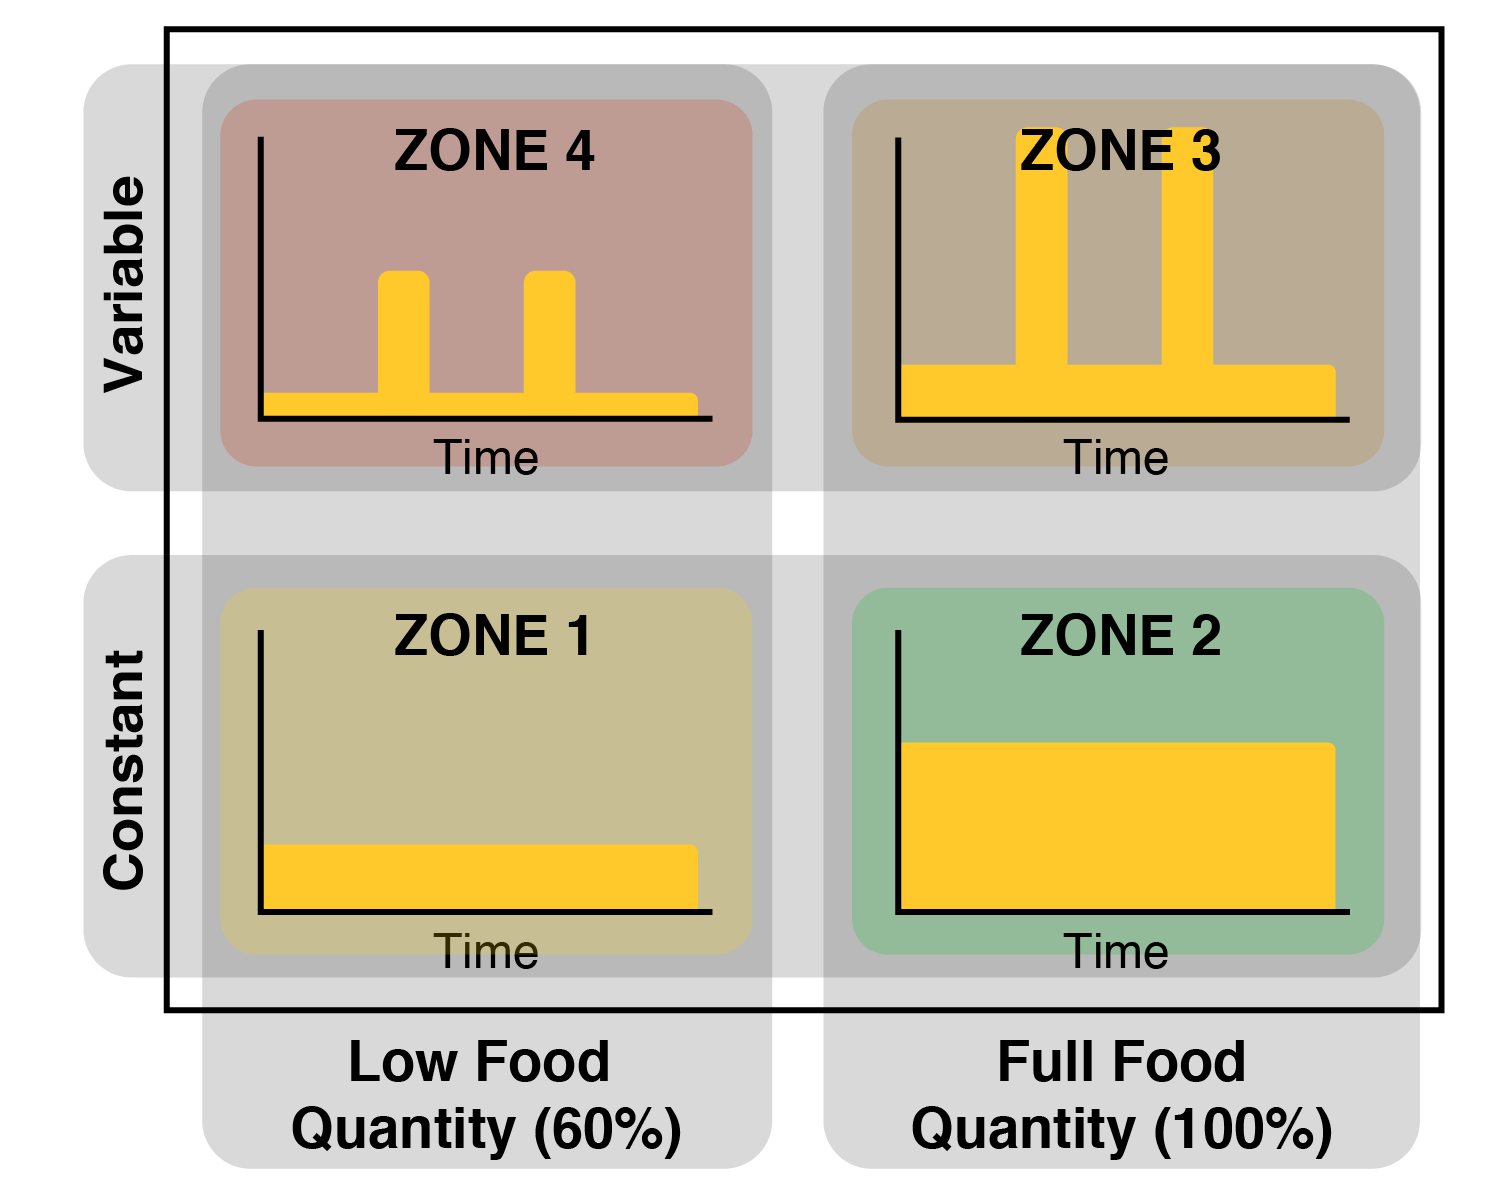
\includegraphics{./fig1_conceptual.png}
\caption{Conceptual depiction of variation in total resource amount as
well as temporal availability. Total resource abundance increases along
the x-axis, while temporal variance increases on the y-axis. We designed
treatments based on the intersecting regions of total food abundance and
temporal availability, with diagrams of food presentation shown in the
inset graphs. The area under the curve in yellow represents the amount
of food presented to bumble bee microcolonies, with both pollen and
nectar following the same pattern. The area under the curve is
equivalent within each food quantity category.}
\end{figure}

\clearpage

\newpage

\begin{figure}
\centering
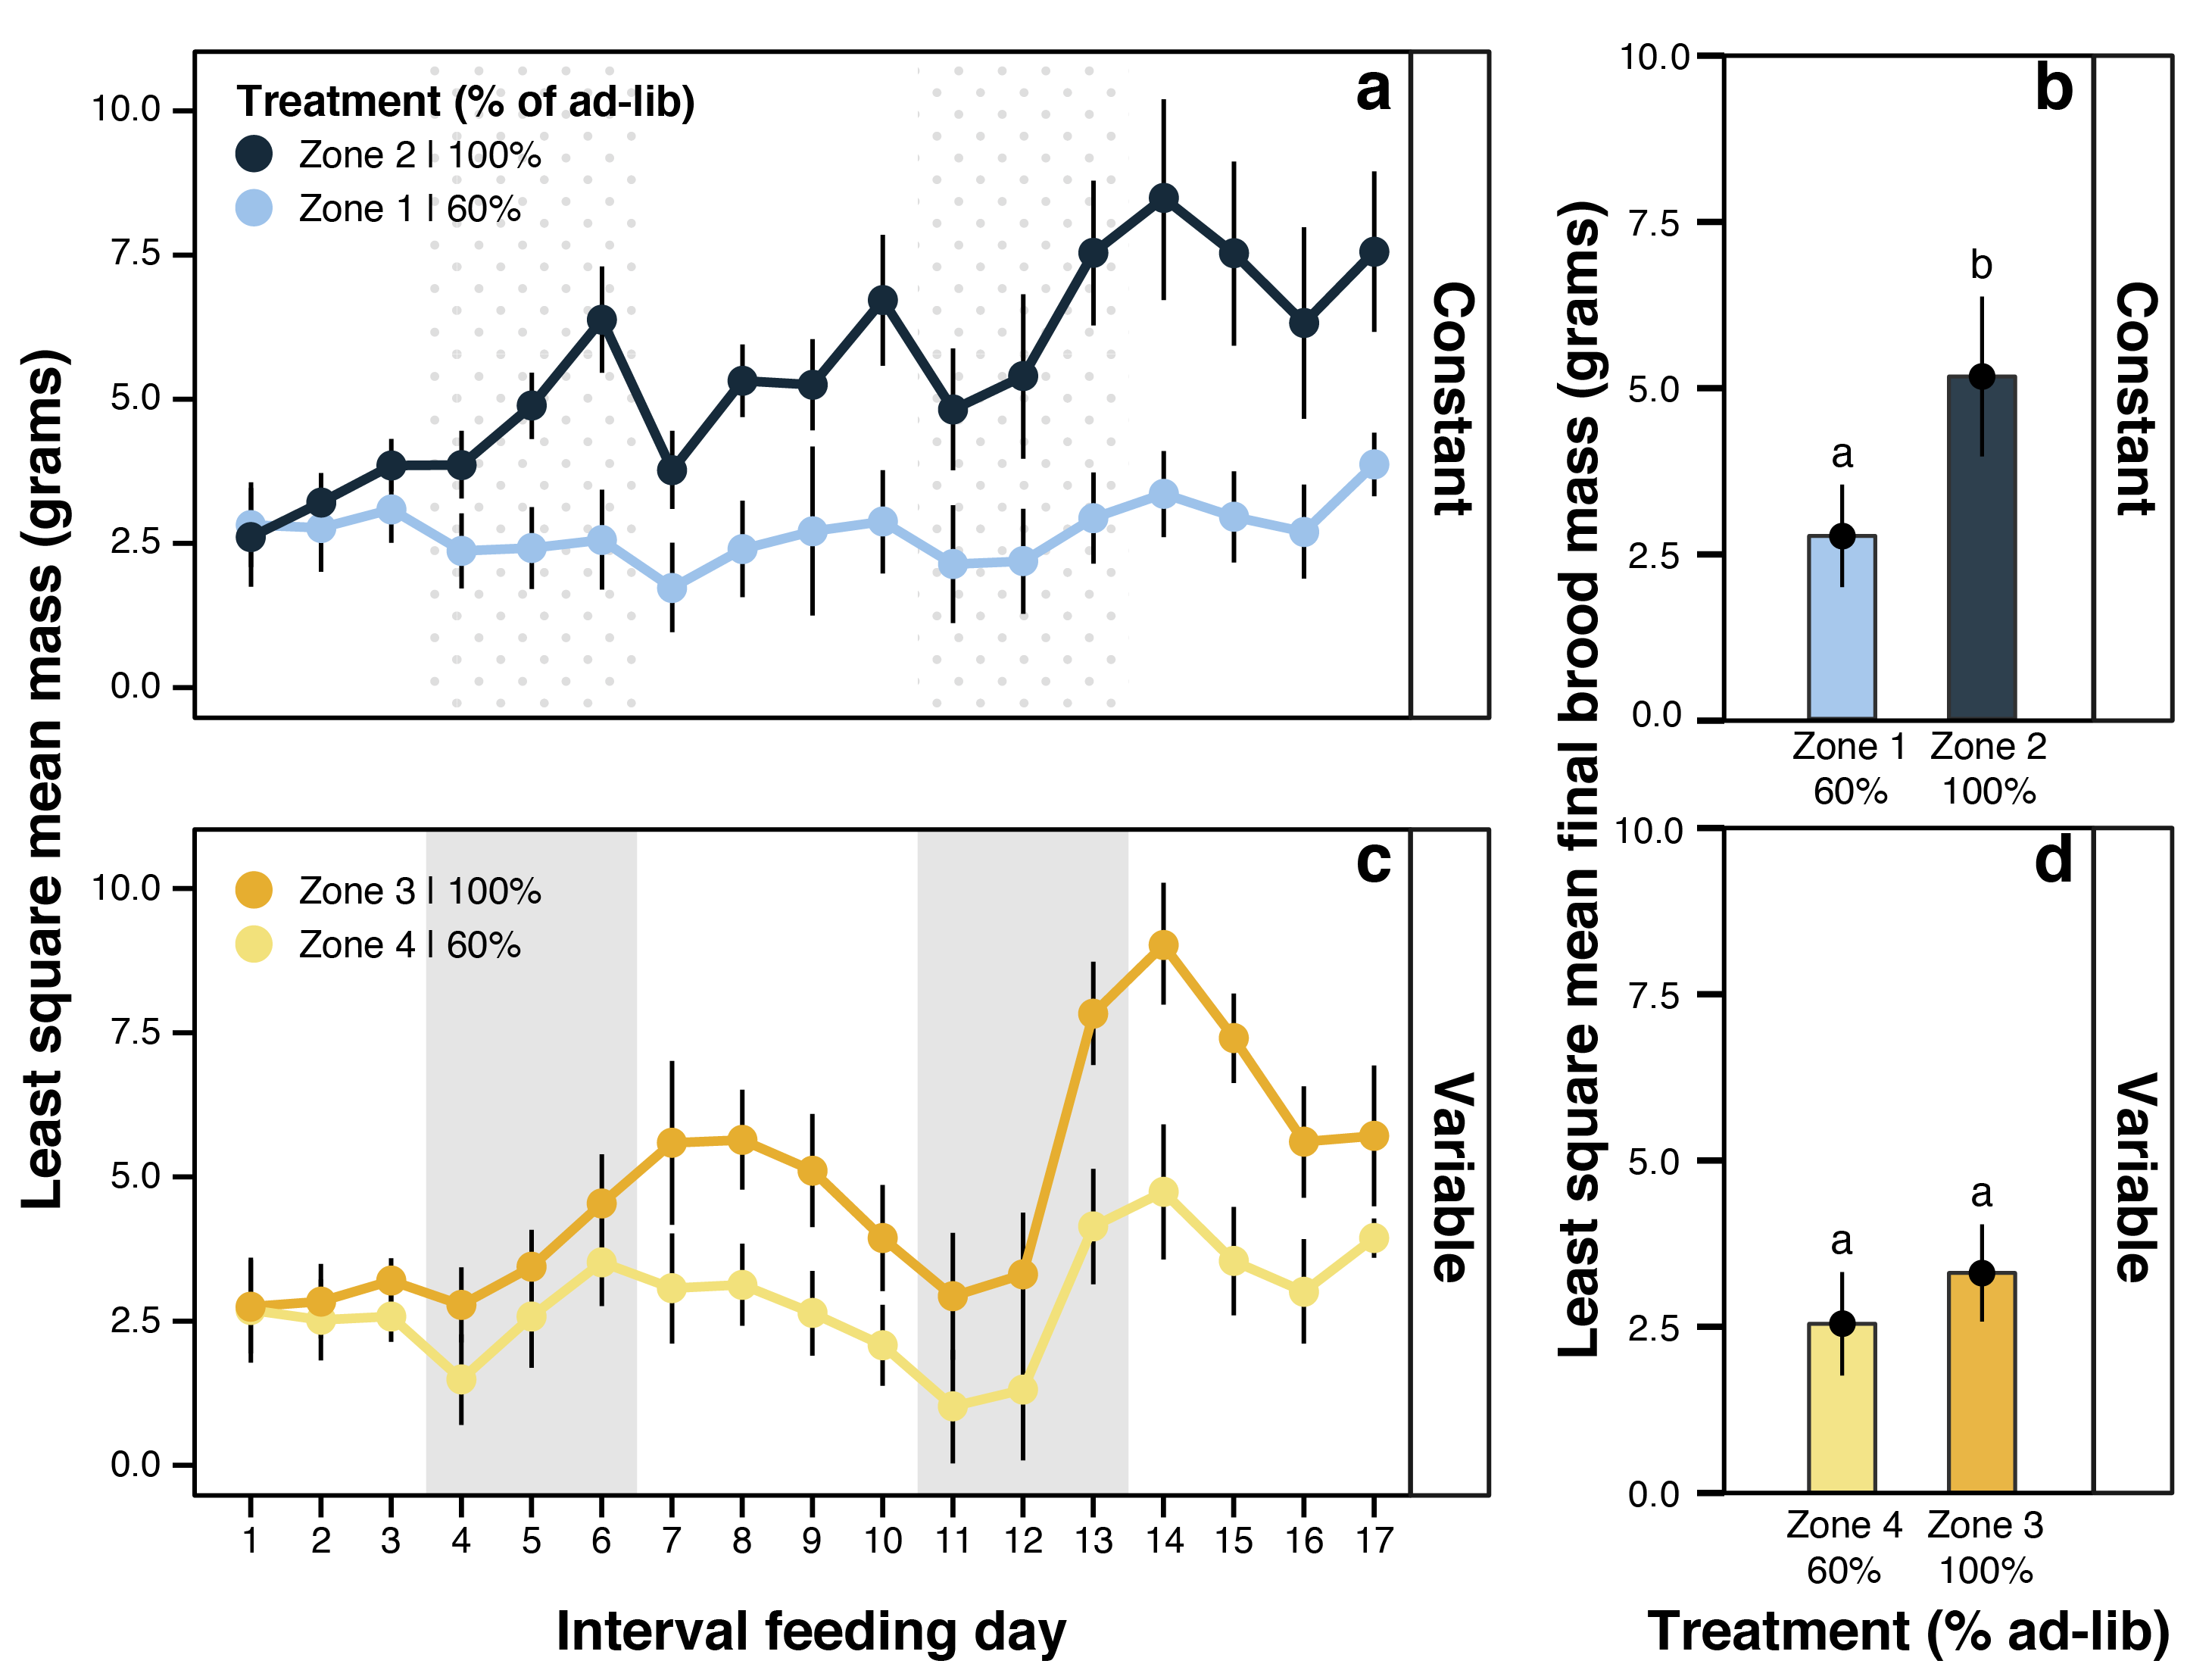
\includegraphics{./fig2_mc_mass.png}
\caption{(a) Least square mean (LSM) estimated mass throughout the
experiment and (b) Least square mean terminal brood mass. Letters
indicate significant differences both within and across temporal
treatment categories (constant and variable). Error bars are 95\%
confidence intervals. Difference of 1 interval feeding day is equal to 3
Julian days.}
\end{figure}

\clearpage

\newpage

\begin{figure}
\centering
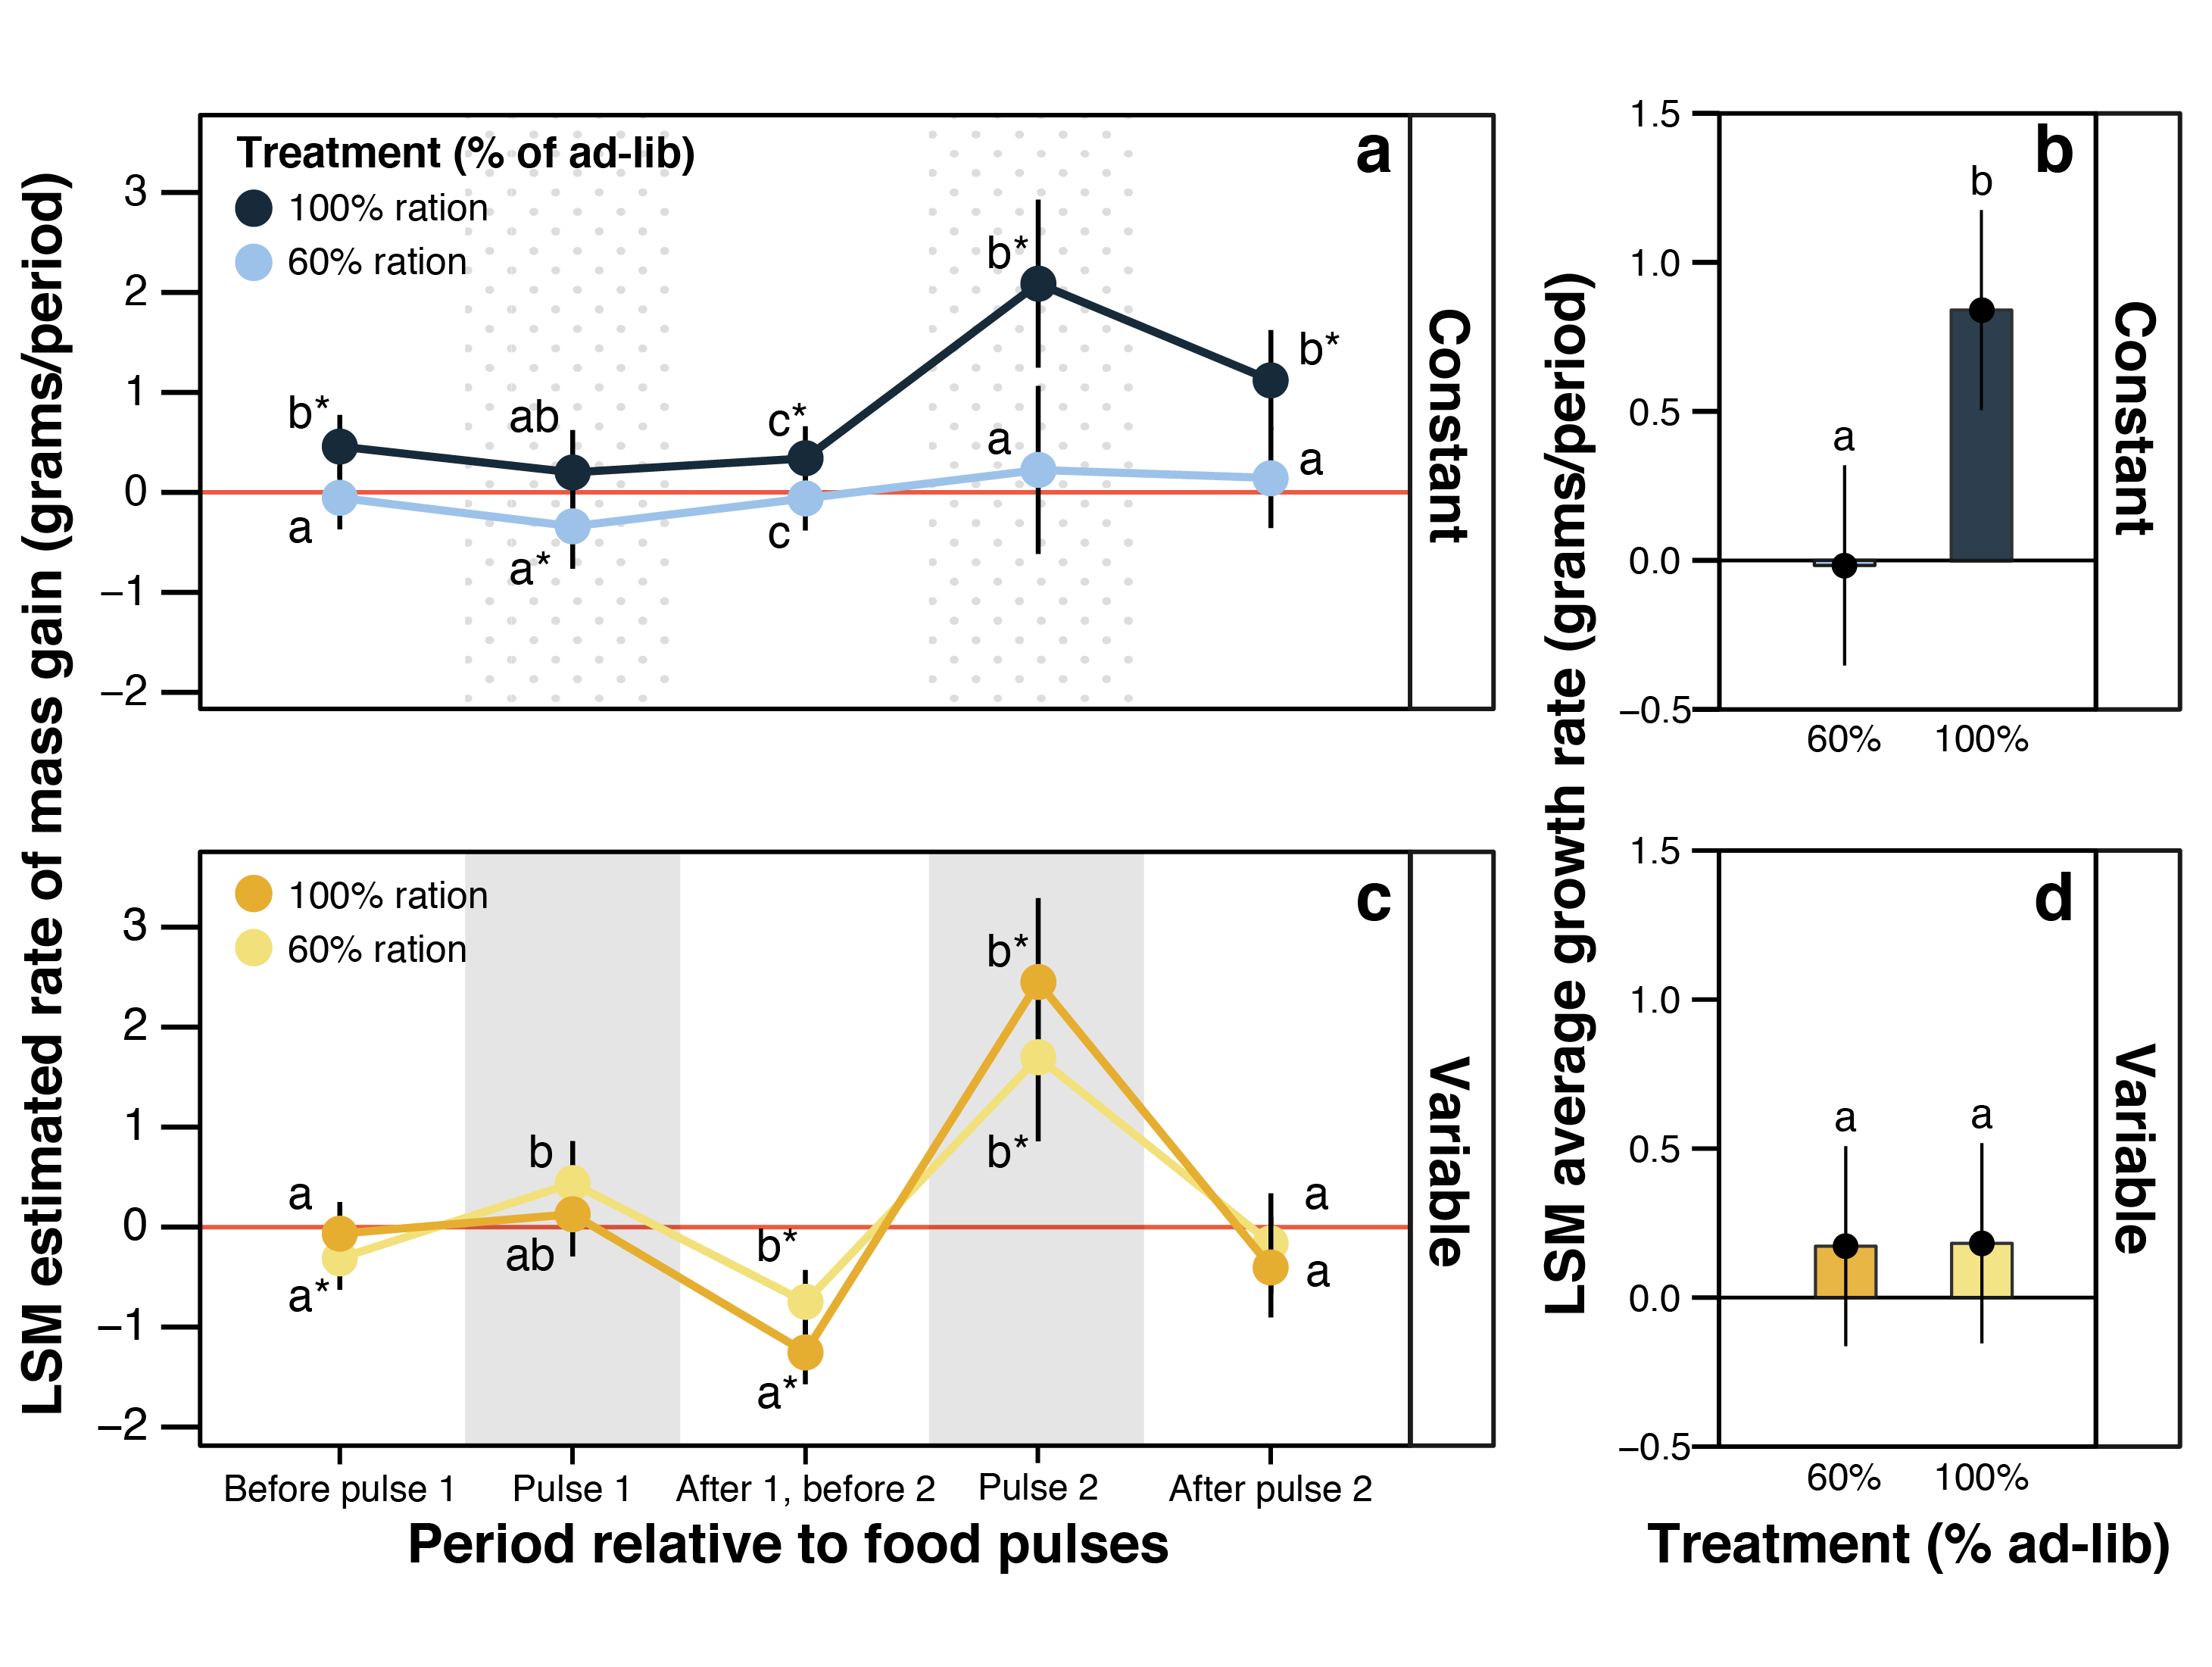
\includegraphics{./fig3_mc_growth.png}
\caption{(a,c) Least square mean (LSM) estimated growth rate by time
periods relative to pulses. Letters indicate significant differences
both within and across temporal treatment categories (constant and
variable) \emph{within periods} (x-axis), and asterisks represent growth
estimates significantly different than 0. Error bars are 95\% confidence
intervals. (b,d) Least square mean growth rates by treatment. Letters
indicate significant differences both within and across temporal
treatments. Error bars are 95\% confidence intervals Difference of 1
interval feeding day is equal to 3 Julian days.}
\end{figure}

\clearpage

\newpage

\begin{figure}
\centering
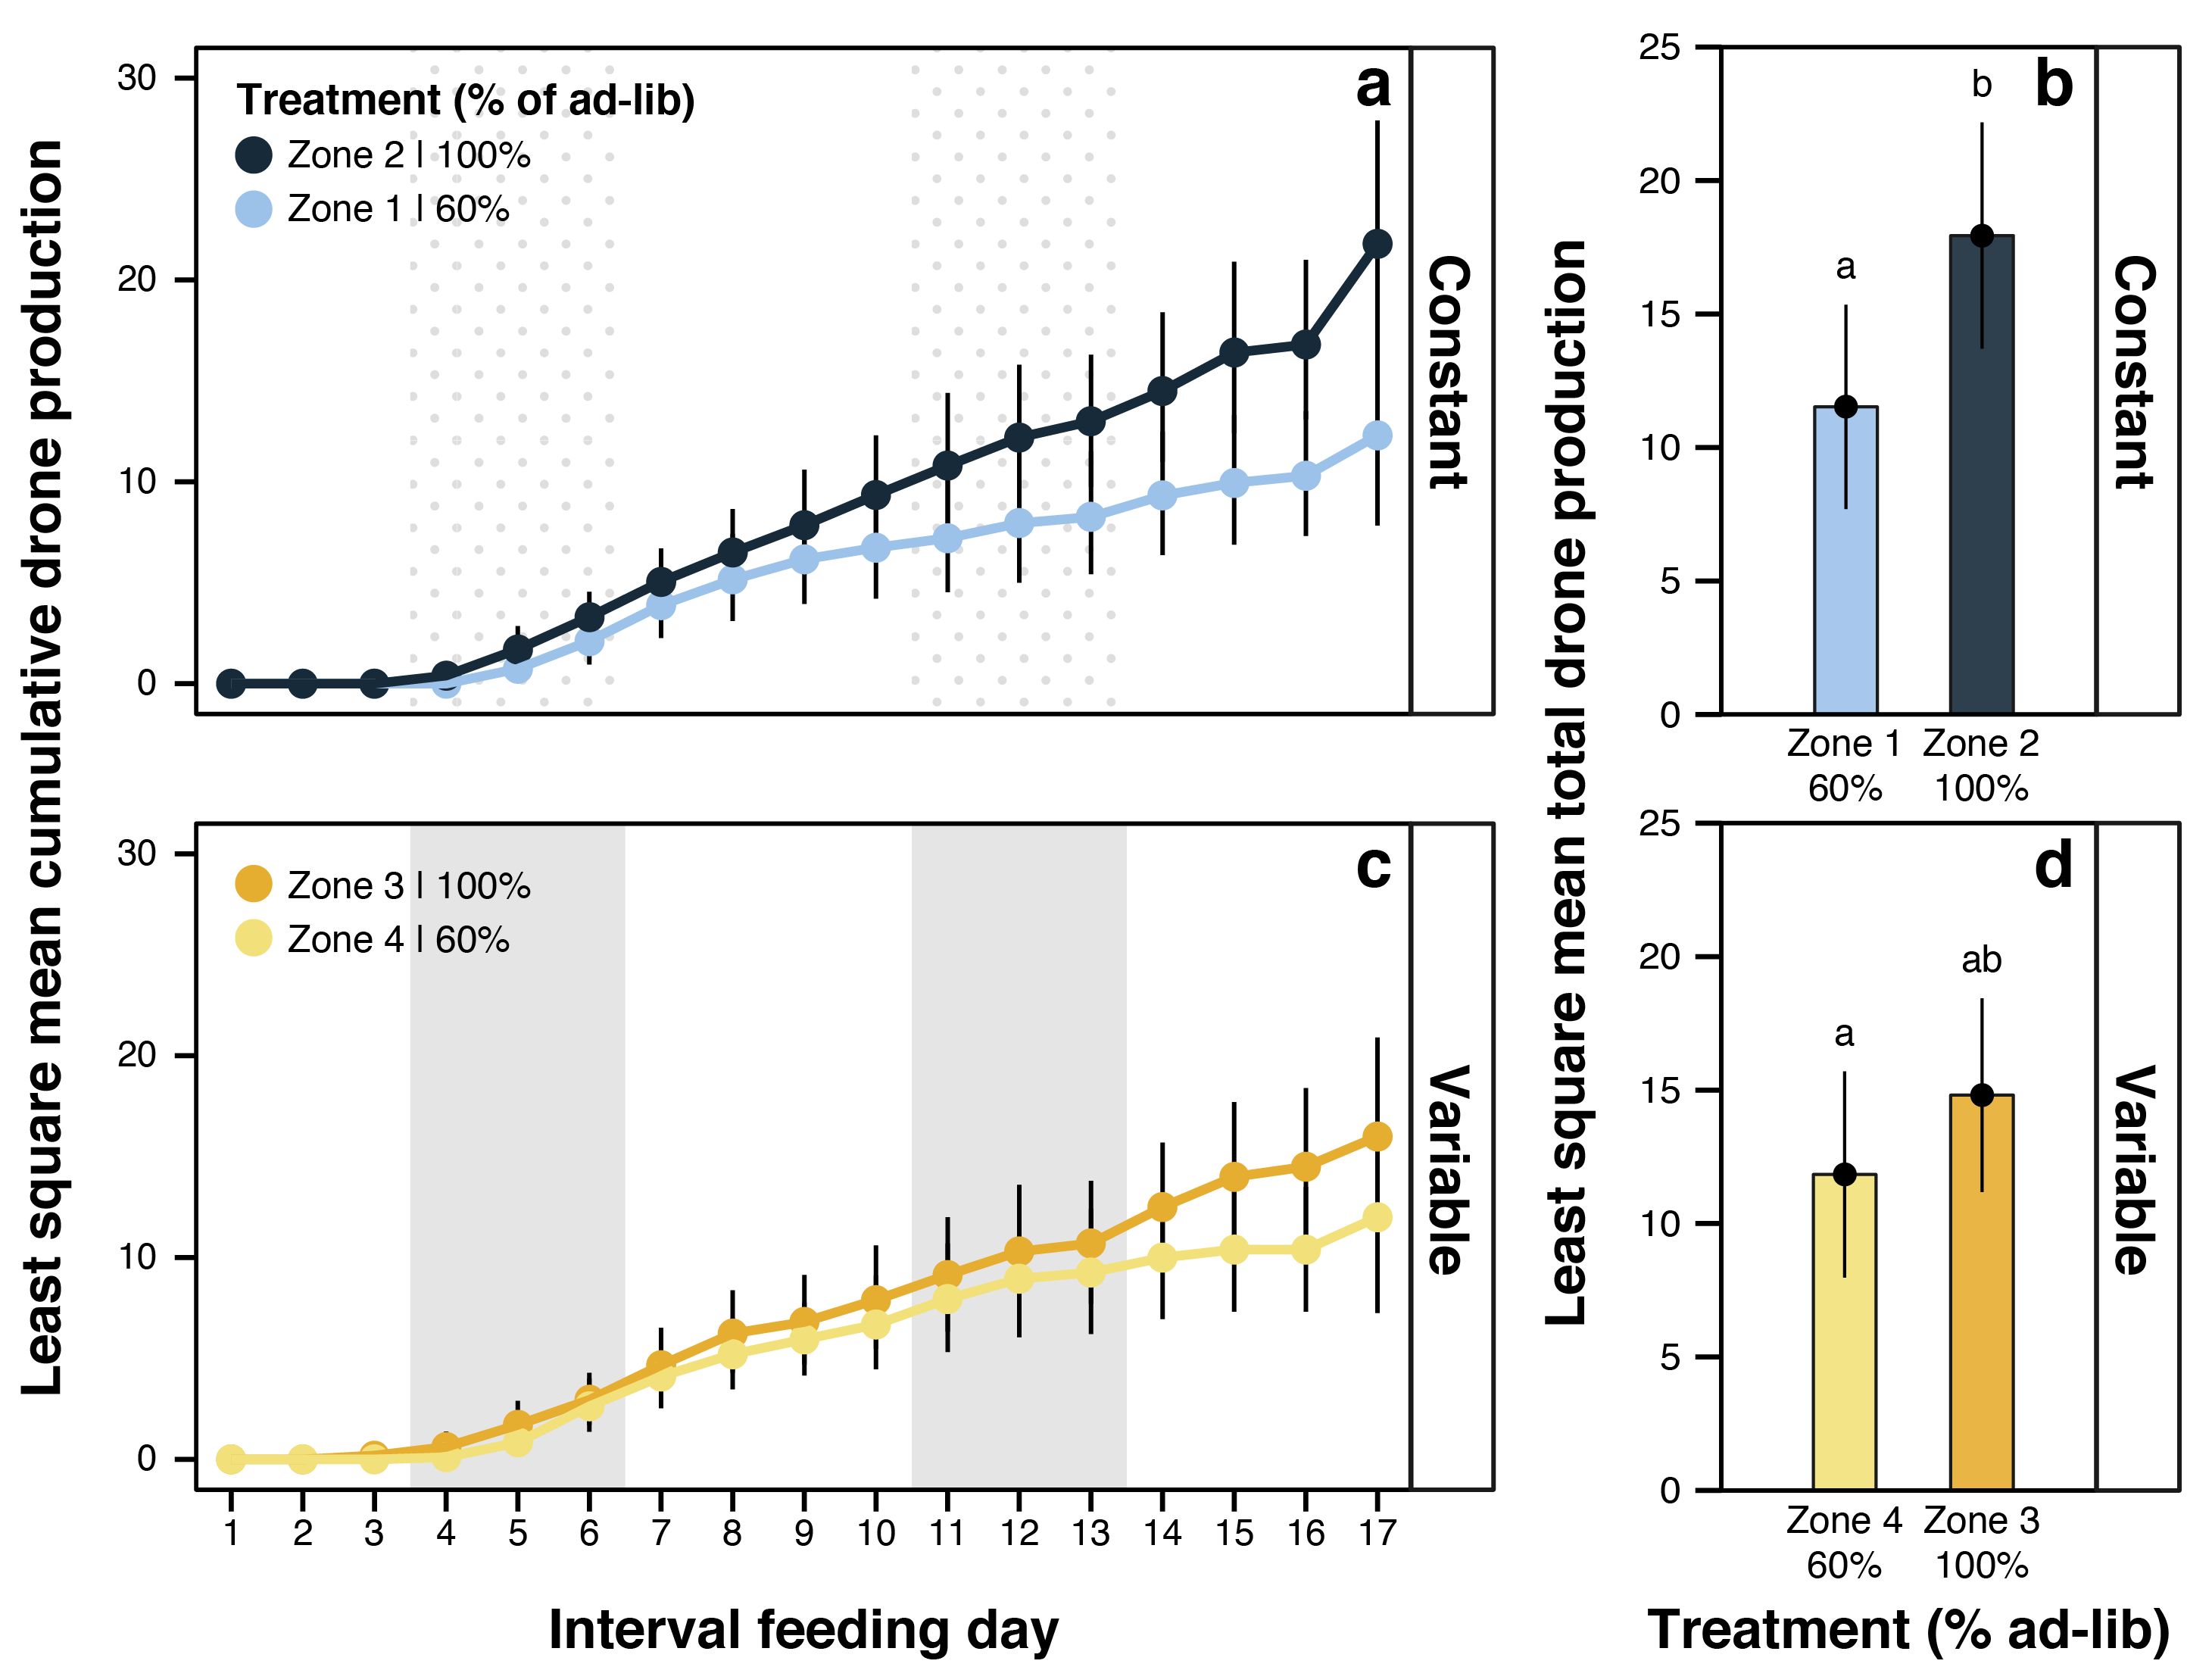
\includegraphics{./fig4_drones.png}
\caption{(a,c) Least square mean (LSM) estimated cumulative drone
production and (b,d) Least square mean total drone production. Letters
indicate significant differences both within and across temporal
treatment categories (constant and variable). Error bars are 95\%
confidence intervals. Difference of 1 interval feeding day is equal to 3
Julian days.}
\end{figure}

\clearpage

\newpage

\hypertarget{references}{%
\section*{References}\label{references}}
\addcontentsline{toc}{section}{References}

\hypertarget{refs}{}
\leavevmode\hypertarget{ref-Benton2003}{}%
Benton, Tim G., Juliet A. Vickery, and Jeremy D. Wilson. 2003.
``Farmland biodiversity: Is habitat heterogeneity the key?''
\emph{Trends Ecol. Evol.} 18 (4): 182--88.
\url{https://doi.org/10.1016/S0169-5347(03)00011-9}.

\leavevmode\hypertarget{ref-Blaauw2014}{}%
Blaauw, Brett R., and Rufus Isaacs. 2014. ``Flower plantings increase
wild bee abundance and the pollination services provided to a
pollination-dependent crop.'' Edited by Yann Clough. \emph{J. Appl.
Ecol.}, April, n/a--n/a. \url{https://doi.org/10.1111/1365-2664.12257}.

\leavevmode\hypertarget{ref-Brown2016a}{}%
Brown, Mark J.F., Lynn V Dicks, Robert J Paxton, Katherine C.R. Baldock,
Andrew B Barron, Marie-pierre Chauzat, Breno M Freitas, et al. 2016. ``A
horizon scan of future threats and opportunities for pollinators and
pollination.'' \emph{PeerJ} 4 (3): e2249.
\url{https://doi.org/10.7717/peerj.2249}.

\leavevmode\hypertarget{ref-Cameron2011}{}%
Cameron, Sydney A, Jeffrey D Lozier, James P Strange, Jonathan B Koch,
Nils Cordes, Leellen F Solter, Terry L Griswold, and Gene E Robinson.
2011. ``Patterns of widespread decline in North American bumble bees.''
\emph{Proc. Natl. Acad. Sci. U. S. A.} 108 (2): 662--67.
\url{https://doi.org/10.1073/pnas.1014743108}.

\leavevmode\hypertarget{ref-Cartar1991}{}%
Cartar, Ralph V., and Lawrence M. Dill. 1991. ``COSTS of Energy
Shortfall for Bumble Bee Colonies: PREDATION, Social Parasitism, and
Brood Development.'' \emph{The Canadian Entomologist} 123 (2): 283--93.
\url{https://doi.org/10.4039/Ent123283-2}.

\leavevmode\hypertarget{ref-Carvell2007}{}%
Carvell, C., W. R. Meek, R. F. Pywell, D. Goulson, and M. Nowakowski.
2007. ``Comparing the efficacy of agri-environment schemes to enhance
bumble bee abundance and diversity on arable field margins.'' \emph{J.
Appl. Ecol.} 44 (1): 29--40.
\url{https://doi.org/10.1111/j.1365-2664.2006.01249.x}.

\leavevmode\hypertarget{ref-Couvillon2010}{}%
Couvillon, M. J., and a. Dornhaus. 2010. ``Small worker bumble bees
(Bombus impatiens) are hardier against starvation than their larger
sisters.'' \emph{Insectes Soc.} 57: 193--97.
\url{https://doi.org/10.1007/s00040-010-0064-7}.

\leavevmode\hypertarget{ref-Crone2016}{}%
Crone, Elizabeth E., Neal M. Williams, and Ecology Letters. 2016.
``Bumble bee colony dynamics: Quantifying the importance of land use and
floral resources for colony growth and queen production.'' Edited by
Rebecca Irwin. \emph{Ecol. Lett.} 19 (4): 460--68.
\url{https://doi.org/10.1111/ele.12581}.

\leavevmode\hypertarget{ref-Dance2017}{}%
Dance, C., C. Botías, and D. Goulson. 2017. ``The combined effects of a
monotonous diet and exposure to thiamethoxam on the performance of
bumblebee micro-colonies.'' \emph{Ecotoxicol. Environ. Saf.} 139
(November 2016): 194--201.
\url{https://doi.org/10.1016/j.ecoenv.2017.01.041}.

\leavevmode\hypertarget{ref-Elliott2009}{}%
Elliott, Susan E. 2009. ``Surplus nectar available for subalpine bumble
bee colony growth.'' \emph{Environ. Entomol.} 38 (6): 1680--9.
\url{https://doi.org/10.1603/022.038.0621}.

\leavevmode\hypertarget{ref-Furst2014}{}%
Fürst, M a, D P McMahon, J L Osborne, R J Paxton, and M J F Brown. 2014.
``Disease associations between honeybees and bumblebees as a threat to
wild pollinators.'' \emph{Nature} 506 (7488): 364--66.
\url{https://doi.org/10.1038/nature12977}.

\leavevmode\hypertarget{ref-Goulson2008}{}%
Goulson, Dave. 2010. \emph{Bumble bees: behavior ecology, and
conservation}. 2nd ed. Oxford University Press.

\leavevmode\hypertarget{ref-Goulson2016}{}%
Goulson, Dave, and Elizabeth Nicholls. 2016. ``The canary in the
coalmine; bee declines as an indicator of environmental health.''
\emph{Sci. Prog.} 99 (3): 312--26.
\url{https://doi.org/10.3184/003685016X14685000479908}.

\leavevmode\hypertarget{ref-Goulson2015c}{}%
Goulson, Dave, Elizabeth Nicholls, C. Botias, Ellen L. Rotheray,
Cristina Botías, and Ellen L. Rotheray. 2015. ``Bee declines driven by
combined stress from parasites, pesticides, and lack of flowers.''
\emph{Science (80-. ).}, no. February: 1--16.
\url{https://doi.org/10.1126/science.1255957}.

\leavevmode\hypertarget{ref-Goulson2002c}{}%
Goulson, D., W. O.H. Hughes, L. C. Derwent, and J. C. Stout. 2002.
``Colony growth of the bumblebee, Bombus terrestris, in improved and
conventional agricultural and suburban habitats.'' \emph{Oecologia} 130
(2): 267--73. \url{https://doi.org/10.1007/s004420100803}.

\leavevmode\hypertarget{ref-Grab2019}{}%
Grab, Heather, Michael G Branstetter, Nolan Amon, Katherine R.
Urban-Mead, Mia G Park, Jason Gibbs, Eleanor J Blitzer, Katja Poveda,
Greg Loeb, and Bryan N Danforth. 2019. ``Agriculturally dominated
landscapes reduce bee phylogenetic diversity and pollination services.''
\emph{Science (80-. ).} 363 (6424): 282--84.
\url{https://doi.org/10.1126/science.aat6016}.

\leavevmode\hypertarget{ref-Greenleaf2007b}{}%
Greenleaf, Sarah S, Neal M Williams, Rachael Winfree, and Claire Kremen.
2007. ``Bee foraging ranges and their relationship to body size.''
\emph{Oecologia} 153 (3): 589--96.
\url{https://doi.org/10.1007/s00442-007-0752-9}.

\leavevmode\hypertarget{ref-Grixti2009}{}%
Grixti, Jennifer C., Lisa T. Wong, Sydney a. Cameron, and Colin Favret.
2009. ``Decline of bumble bees (Bombus) in the North American Midwest.''
\emph{Biol. Conserv.} 142 (1): 75--84.
\url{https://doi.org/10.1016/j.biocon.2008.09.027}.

\leavevmode\hypertarget{ref-Hass2018a}{}%
Hass, Annika Louise, Lara Brachmann, Péter Batáry, Yann Clough, Hermann
Behling, and Teja Tscharntke. 2018. ``Maize-dominated landscapes reduce
bumblebee colony growth through pollen diversity loss.'' \emph{J. Appl.
Ecol.}, no. September: 1--11.
\url{https://doi.org/10.1111/1365-2664.13296}.

\leavevmode\hypertarget{ref-Heinrich2004}{}%
Heinrich, Bernd. 2004. \emph{Bumblebee Economics}. Harvard University
Press.

\leavevmode\hypertarget{ref-Hines2005}{}%
Hines, Heather M, and Stephen D Hendrix. 2005. ``Bumble Bee (
Hymenoptera : Apidae ) Diversity and Abundance in Tallgrass Prairie
Patches : Effects of Local and Landscape Floral Resources.'' \emph{Env.
. Entomol} 34 (6): 1477--84.
\url{https://doi.org/10.1603/0046-225X-34.6.1477}.

\leavevmode\hypertarget{ref-Holzschuh2013}{}%
Holzschuh, Andrea, Carsten F. Dormann, Teja Tscharntke, and Ingolf
Steffan-Dewenter. 2013. ``Mass-flowering crops enhance wild bee
abundance.'' \emph{Oecologia} 172 (2): 477--84.
\url{https://doi.org/10.1007/s00442-012-2515-5}.

\leavevmode\hypertarget{ref-multcomp}{}%
Hothorn, Torsten, Frank Bretz, and Peter Westfall. 2008. ``Simultaneous
Inference in General Parametric Models.'' \emph{Biometrical Journal} 50
(3): 346--63.

\leavevmode\hypertarget{ref-Jacobson2018a}{}%
Jacobson, Molly M., Erika M. Tucker, Minna E. Mathiasson, and Sandra M.
Rehan. 2018. ``Decline of bumble bees in northeastern North America,
with special focus on Bombus terricola.'' \emph{Biol. Conserv.} 217
(August 2017): 437--45.
\url{https://doi.org/10.1016/j.biocon.2017.11.026}.

\leavevmode\hypertarget{ref-Junker2010}{}%
Junker, Robert R., and Nico Blüthgen. 2010. ``Floral scents repel
facultative flower visitors, but attract obligate ones.'' \emph{Ann.
Bot.} 105 (5): 777--82. \url{https://doi.org/10.1093/aob/mcq045}.

\leavevmode\hypertarget{ref-Kerr2015}{}%
Kerr, Jeremy T, Alana Pindar, Paul Galpern, Laurence Packer, Simon G
Potts, Stuart M Roberts, Pierre Rasmont, et al. 2015. ``Climate change
impacts on bumblebees converge across continents.'' \emph{Science (80-.
).} 349 (6244): 177--80. \url{https://doi.org/10.1126/science.aaa7031}.

\leavevmode\hypertarget{ref-Landis2017}{}%
Landis, Douglas A. 2017. ``Designing agricultural landscapes for
biodiversity-based ecosystem services.'' \emph{Basic Appl. Ecol.} 18:
1--12. \url{https://doi.org/10.1016/j.baae.2016.07.005}.

\leavevmode\hypertarget{ref-emmeans}{}%
Lenth, Russell. 2019. \emph{Emmeans: Estimated Marginal Means, Aka
Least-Squares Means}. \url{https://CRAN.R-project.org/package=emmeans}.

\leavevmode\hypertarget{ref-lsmeans}{}%
Lenth, Russell V. 2016. ``Least-Squares Means: The R Package lsmeans.''
\emph{Journal of Statistical Software} 69 (1): 1--33.
\url{https://doi.org/10.18637/jss.v069.i01}.

\leavevmode\hypertarget{ref-Martins2018}{}%
Martins, Kyle T., Cécile H. Albert, Martin J. Lechowicz, and Andrew
Gonzalez. 2018. ``Complementary crops and landscape features sustain
wild bee communities.'' \emph{Ecol. Appl.} 28 (4): 1093--1105.
\url{https://doi.org/10.1002/eap.1713}.

\leavevmode\hypertarget{ref-McArt2017}{}%
McArt, Scott H., Christine Urbanowicz, Shaun McCoshum, Rebecca E. Irwin,
and Lynn S. Adler. 2017. ``Landscape predictors of pathogen prevalence
and range contractions in US bumblebees.'' \emph{Proc. R. Soc. B Biol.
Sci.} 284 (1867): 20172181.
\url{https://doi.org/10.1098/rspb.2017.2181}.

\leavevmode\hypertarget{ref-Moerman2017}{}%
Moerman, Romain, Maryse Vanderplanck, Denis Fournier, Anne Laure
Jacquemart, and Denis Michez. 2017. ``Pollen nutrients better explain
bumblebee colony development than pollen diversity.'' \emph{Insect
Conserv. Divers.} 10 (2): 171--79.
\url{https://doi.org/10.1111/icad.12213}.

\leavevmode\hypertarget{ref-Peat2005}{}%
Peat, J., J. Tucker, and Dave Goulson. 2005. ``Does intraspecific size
variation in bumblebees allow colonies to efficiently exploit different
flowers?'' \emph{Ecol. Entomol.} 30 (2): 176--81.
\url{https://doi.org/10.1111/j.0307-6946.2005.00676.x}.

\leavevmode\hypertarget{ref-Pelletier2003}{}%
Pelletier, Luc, and Jeremy N McNeil. 2003. ``The effect of food
supplementation on reproductive success in bumblebee field colonies.''
\emph{Oikos} 3 (3): 688--94.
\url{https://doi.org/10.1034/j.1600-0706.2003.12592.x}.

\leavevmode\hypertarget{ref-nlme}{}%
Pinheiro, Jose, Douglas Bates, Saikat DebRoy, Deepayan Sarkar, and R
Core Team. 2018. \emph{nlme: Linear and Nonlinear Mixed Effects Models}.
\url{https://CRAN.R-project.org/package=nlme}.

\leavevmode\hypertarget{ref-rcite}{}%
R Core Team. 2019. \emph{R: A Language and Environment for Statistical
Computing}. Vienna, Austria: R Foundation for Statistical Computing.
\url{https://www.R-project.org/}.

\leavevmode\hypertarget{ref-Rhemtulla2007}{}%
Rhemtulla, Jeanine M., David J. Mladenoff, and Murray K. Clayton. 2007.
``Regional land-cover conversion in the U.S. upper Midwest: Magnitude of
change and limited recovery (1850-1935-1993).'' \emph{Landsc. Ecol.} 22
(SUPPL. 1): 57--75. \url{https://doi.org/10.1007/s10980-007-9117-3}.

\leavevmode\hypertarget{ref-Rotheray2017}{}%
Rotheray, Ellen L, Juliet L Osborne, and Dave Goulson. 2017.
``Quantifying the food requirements and effects of food stress on bumble
bee colony development.'' \emph{J. Apic. Res.} 56 (3): 288--99.
\url{https://doi.org/10.1080/00218839.2017.1307712}.

\leavevmode\hypertarget{ref-Roulston2011}{}%
Roulston, T'ai H, and Karen Goodell. 2011. ``The role of resources and
risks in regulating wild bee populations.'' \emph{Annu. Rev. Entomol.}
56 (August): 293--312.
\url{https://doi.org/10.1146/annurev-ento-120709-144802}.

\leavevmode\hypertarget{ref-Rundlof2014}{}%
Rundlöf, Maj, Anna S. Persson, Henrik G. Smith, and Riccardo Bommarco.
2014. ``Late-season mass-flowering red clover increases bumble bee queen
and male densities.'' \emph{Biol. Conserv.} 172: 138--45.
\url{https://doi.org/10.1016/j.biocon.2014.02.027}.

\leavevmode\hypertarget{ref-Schellhorn2015c}{}%
Schellhorn, Nancy A., Vesna Gagic, and Riccardo Bommarco. 2015. ``Time
will tell: Resource continuity bolsters ecosystem services.''
\emph{Trends Ecol. Evol.} 30 (9): 524--30.
\url{https://doi.org/10.1016/j.tree.2015.06.007}.

\leavevmode\hypertarget{ref-Schluns2003}{}%
Schlüns, Helge, Ellen A. Schlüns, Job van Praagh, and Robin F.A. Moritz.
2003. ``Sperm numbers in drone honeybees ( Apis mellifera ) depend on
body size.'' \emph{Apidologie} 34 (6): 577--84.
\url{https://doi.org/10.1051/apido:2003051}.

\leavevmode\hypertarget{ref-Schmid-Hempel1998a}{}%
Schmid-Hempel, Regula, and Paul Schmid-Hempel. 1998. ``Colony
performance and immunocompetence of a social insect, Bombus terrestris,
in poor and variable environments.'' \emph{Funct. Ecol.} 12 (1): 22--30.
\url{https://doi.org/10.1046/j.1365-2435.1998.00153.x}.

\leavevmode\hypertarget{ref-Senapathi2015a}{}%
Senapathi, Deepa, Luisa G. Carvalheiro, Jacobus C. Biesmeijer,
Cassie-Ann Dodson, Rebeca L. Evans, Megan McKerchar, R. Daniel Morton,
et al. 2015. ``The impact of over 80 years of land cover changes on bee
and wasp pollinator communities in England.'' \emph{Proc. R. Soc. B
Biol. Sci.} 282 (1806): 8. \url{https://doi.org/10.1098/rspb.2015.0294}.

\leavevmode\hypertarget{ref-Smith1998}{}%
Smith, Daryl D. 1998. ``Iowa prairie: Original extent and loss,
preservation and recovery attempts.'' \emph{J. Iowa Acad. Sci.} 105 (3):
94--108.

\leavevmode\hypertarget{ref-Spiesman2017}{}%
Spiesman, Brian J., Ashley Bennett, Rufus Isaacs, and Claudio Gratton.
2017. ``Bumble bee colony growth and reproduction depend on local flower
dominance and natural habitat area in the surrounding landscape.''
\emph{Biol. Conserv.} 206 (February): 217--23.
\url{https://doi.org/10.1016/j.biocon.2016.12.008}.

\leavevmode\hypertarget{ref-Sutcliffe1988}{}%
Sutcliffe, G.H., and R.C. Plowright. 1988. ``THE Effects of Food Supply
on Adult Size in the Bumble Bee Bombus Terricola Kirby (Hymenoptera:
APIDAE).'' \emph{The Canadian Entomologist} 120 (12): 1051--8.
\url{https://doi.org/10.4039/Ent1201051-12}.

\leavevmode\hypertarget{ref-Tasei2008}{}%
Tasei, Jean-Noël, and Pierrick Aupinel. 2008. ``Validation of a method
using queenless Bombus terrestris micro-colonies for testing the
nutritive value of commercial pollen mixes by comparison with queenright
colonies.'' \emph{J. Econ. Entomol.} 101 (6): 1737--42.
\url{https://doi.org/10.1603/0022-0493-101.6.1737}.

\leavevmode\hypertarget{ref-VanderWall1990}{}%
Vander Wall, Stephen B. 1990. ``Food hoarding in animals.''

\leavevmode\hypertarget{ref-Vaudo2018}{}%
Vaudo, Anthony D, Liam M Farrell, Harland M Patch, Christina M
Grozinger, and John F Tooker. 2018. ``Consistent pollen nutritional
intake drives bumble bee ( Bombus impatiens ) colony growth and
reproduction across different habitats.'' \emph{Ecol. Evol.} 8 (11):
5765--76. \url{https://doi.org/10.1002/ece3.4115}.

\leavevmode\hypertarget{ref-Westphal2009a}{}%
Westphal, C., I. Steffan-Dewenter, and T. Tscharntke. 2009. ``Mass
flowering oilseed rape improves early colony growth but not sexual
reproduction of b1. Westphal, C., Steffan-Dewenter, I. \& Tscharntke, T.
(2009). Mass flowering oilseed rape improves early colony growth but not
sexual reproduction of bumblebees. J.'' \emph{J. Appl. Ecol.} 46 (1):
187--93. \url{https://doi.org/10.1111/j.1365-2664.2008.01580.x}.

\leavevmode\hypertarget{ref-Williams2012b}{}%
Williams, Neal M., James Regetz, and Claire Kremen. 2012.
``Landscape-scale resources promote colony growth but not reproductive
performance of bumble bees.'' \emph{Ecology} 93 (5): 1049--58.
\url{https://doi.org/10.1890/11-1006.1}.

\leavevmode\hypertarget{ref-Wood2019}{}%
Wood, Thomas J., Jason Gibbs, Kelsey K. Graham, and Rufus Isaacs. 2019.
``Narrow pollen diets are associated with declining Midwestern bumble
bee species.'' \emph{Ecology} 0 (0).
\url{https://doi.org/10.1002/ecy.2697}.

\leavevmode\hypertarget{ref-Woodard2017}{}%
Woodard, S. Hollis, and Shalene Jha. 2017. ``Wild bee nutritional
ecology: predicting pollinator population dynamics, movement, and
services from floral resources.'' \emph{Curr. Opin. Insect Sci.} 21
(Figure 1): 83--90. \url{https://doi.org/10.1016/j.cois.2017.05.011}.

\leavevmode\hypertarget{ref-zoo}{}%
Zeileis, Achim, and Gabor Grothendieck. 2005. ``Zoo: S3 Infrastructure
for Regular and Irregular Time Series.'' \emph{Journal of Statistical
Software} 14 (6): 1--27. \url{https://doi.org/10.18637/jss.v014.i06}.


\end{document}
